\documentclass[article,12pt]{article}

\usepackage[utf8]{inputenc}
\usepackage{amssymb, amsfonts,amsthm}
\usepackage[fleqn]{amsmath} % Math packages
\numberwithin{equation}{section}
\usepackage{listings}
\usepackage[top=1in, bottom=1in, left=1in, right=1in]{geometry}
%\usepackage[T1]{fontenc} % Use 8-bit encoding that has 256 glyphs
%\usepackage{fourier} % Use the Adobe Utopia font for the document - comment this line to return to the LaTeX default
\usepackage[english]{babel} % English language/hyphenation
\usepackage{enumerate}
\usepackage[usenames,dvipsnames]{color} % Required for custom colors
\usepackage{listings} % Required for insertion of code
\usepackage{courier} % Required for the courier font
\usepackage{tikz} 
\usepackage{sectsty}
\usepackage{multicol} % Required for multiple columns
%\usepackage{tabu} % Option for Table Construction
\usepackage{epigraph} 
\setlength{\epigraphwidth}{\textwidth}
\usepackage{hologo}
\usepackage[font=small,labelfont=bf]{caption} % Specifying Captions
\usepackage{multirow} % TAbles
\usepackage{changepage} % Change margins



\usepackage{blindtext}
\usepackage{setspace} % Spacing
\usepackage{csquotes}% Recommended
\usepackage{psvectorian} % Cool ornaments

\usepackage{hyperref} % hyper links
\hypersetup{
	colorlinks=true,
	linkcolor=blue,
	filecolor=magenta,      
	urlcolor=cyan,
	pdftitle={Prospectus},
	pdfpagemode=FullScreen,
	citecolor= black
}

\urlstyle{same}


\renewcommand{\baselinestretch}{1.5} % Spacing

\usepackage[style = numeric, sorting = none, backend=biber]{biblatex}
\addbibresource{references.bib}

\usepackage{graphicx}
\graphicspath{{figs/}} %Setting the graphicspath


\begin{document}

\begin{center}
Lab Report

Title: Lab1\\
Notice: Dr. Bryan Runck\\
Author: Rob Hendrickson\\
Date: 10/9/2022\\~\\

Repository: \url{https://github.com/RwHendrickson/GIS5571/tree/main/Lab01}\\
Time Spent: 15 hours

\end{center}

\section*{Abstract}
In this lab, I explored 3 different spatial web API's and how to make them interoperable. The problem statement section explains why this is an important skill for a GIS professional as well as the general workflow of this assignment. The input data section will describe the different datasets acquired in this exercise. The methods section includes detailed visual and textual descriptions of the workflow conducted. The results section will present some visualizations showing the datasets that were created. This report concludes with a discussion on the different API conceptual models and their pros and cons.


\section*{Problem Statement}
Web API's are a way for data scientists to programatically acquire information for their analyses. One challenge with this process is that there is not a standardized way to design an API. Furthermore, when spatial information is included, the format in which it is returned varies significantly. This lab compares three spatial web API's: Minnesota Geospatial Commons, Google Places, and North Dakota Agricultural Weather Newtowrk (NDAWN). After growing familiar with each interface, an ETL routine is developed which makes the datasets interoperable. We conclude by spatially joining information between each API and saving the integrated data to an ESRI geodatabase. 

\fbox{ % Workflow
	\begin{minipage}{.8\linewidth}
		\begin{center}
			\begin{minipage}{\linewidth}
				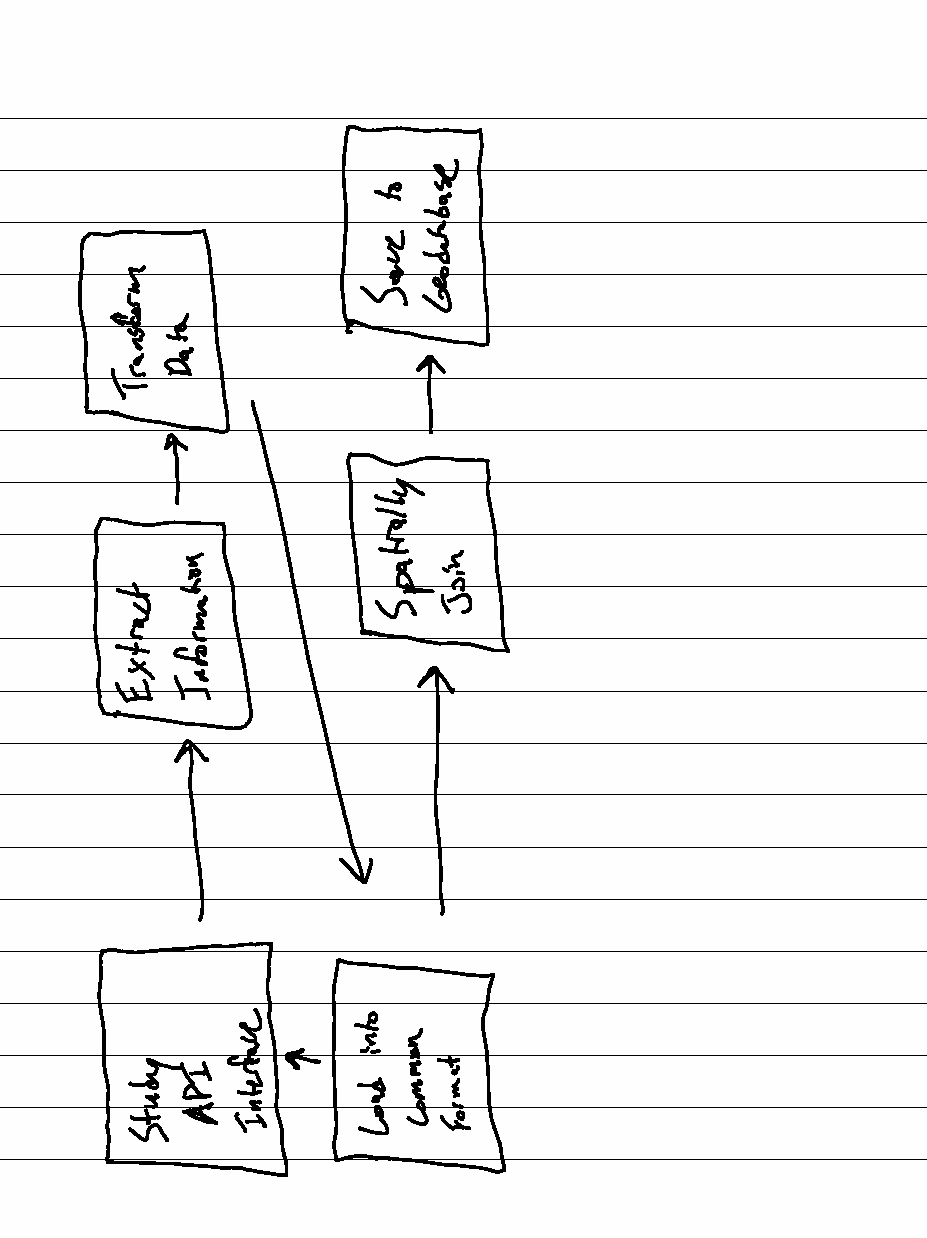
\includegraphics[width=.75\linewidth,angle=270]{steps}
			\end{minipage}
			\captionof{figure}{General Steps}
		\end{center}
	\end{minipage}
}\\
{
	\scriptsize
	\begin{tabular}{|l|p{.12\linewidth}|p{.2\linewidth}|p{.2\linewidth}|p{.1\linewidth}|p{.1\linewidth}|p{.1\linewidth}|}
	\hline	& \textbf{Requirement} & \textbf{Defined As} & \textbf{(Spatial) Data} & \textbf{Attribute Data} & \textbf{Dataset} & \textbf{Preparation} \\ \hline
		1 &  Study Minnesota Geospatial Commons API       &    Explore interface, extract data, transform                                                            & Road Geometry | Municipal Boundaries         &   Traffic Volume Counts | Boundary Names                                               & \href{https://gisdata.mn.gov/dataset/trans-aadt-traffic-segments}{Minnesota Dept. of Transportation} | \href{https://gisdata.mn.gov/dataset/us-mn-state-metc-bdry-census2010counties-ctus}{Metropolitan Council}                                                                                                                &       Navigated the MN Geospatial Commons Website \\ \hline
		2 &  Study Google Places API       &    Explore interface, extract data, transform                                                            & Pools Point Geometry | Schools Point Geometry         &   Address, names, business status, rating, etc.                                   &                                                                                                               & Create Google API Key  \\ \hline
		3 &  Study NDAWN API       &    Explore interface, extract data, transform                                                            & Station Point Geometry         &  Month, Year, Min/Max/Avg. Temperature                                               &                                                                                                                &       Navigated the NDAWN website \\ \hline
		4 & Synthesize Data                            & Ensure that datasets are in the same CRS and spatially join &                   &                                                   &                                                                                                                                           &             \\ \hline
		5 & Save synthesized data & Save to a common geodatabase                &                                         &                                                   &                                                                                                                                                                                                         &             \\ \hline     
	\end{tabular}
\captionof{table}{Project Steps}}

\section*{Input Data}
The data acquired from the Geospatial Commons was Minnesota Department of Transportation (MnDoT) current annual average daily traffic (AADT) of all the roads of Minnesota and the Metropolitan Council's (MetCouncil) city and township (CTU) boundaries. Information acquired from Google Places was the primary schools nearby the intersection of the 94 and 35W interstate highways and municipal pools in North Dakota. From NDAWN, monthly maximum, minimum, and average temperatures were acquired for all weather stations for the past year. Their API links can be found in the following table. \vspace{.5in}

{
	\scriptsize
	\begin{tabular}{|l|p{.2\linewidth}|p{.2\linewidth}|p{.4\linewidth}|}
	& \textbf{Title}                              & \textbf{Purpose in Analysis}     & \textbf{Link to Source} \\ \hline
	1 & MetCouncil’s CTU's & Joining with Road Network & \url{https://gisdata.mn.gov/dataset/us-mn-state-metc-bdry-census2010counties-ctus }        \\                 
	2 & MnDoT’s Current AADT Segments     & Joining with CTU's and Schools & \url{https://gisdata.mn.gov/dataset/trans-aadt-traffic-segments}                   \\
	3 & Schools in Minneapolis     & Joining with Roads        & \url{https://maps.googleapis.com/maps/api/place/nearbysearch/json?location=44.965676%2C-93.259512&rankby=distance&type=primary_school&keyword=school}                                                   \\
	4 & Pools in North Dakota                        & Joining with Weather Stations             & \url{https://maps.googleapis.com/maps/api/place/textsearch/json?input=Municipal%20Pool%20in%20North%20Dakota&inputtype=textquery&locationbias=rectangle:45.951407,-104.048971|49,-96.561788}                                              \vspace{.1in} \\
	5 & Max/Min/Avg. Temps across North Dakota (Past year)                       & Joining with Pools              &   \href{https://ndawn.ndsu.nodak.edu/table.csv?station=78&station=111&station=98&station=174&station=142&station=138&station=161&station=9&station=10&station=118&station=56&station=11&station=12&station=58&station=13&station=84&station=55&station=7&station=87&station=14&station=15&station=96&station=16&station=137&station=124&station=143&station=17&station=85&station=140&station=134&station=18&station=136&station=65&station=104&station=99&station=19&station=129&station=20&station=101&station=81&station=21&station=97&station=22&station=75&station=2&station=172&station=139&station=23&station=62&station=86&station=24&station=89&station=126&station=93&station=90&station=25&station=83&station=107&station=156&station=77&station=26&station=70&station=127&station=27&station=132&station=28&station=29&station=30&station=31&station=102&station=32&station=119&station=4&station=80&station=33&station=59&station=105&station=82&station=34&station=72&station=135&station=35&station=76&station=120&station=141&station=109&station=36&station=79&station=71&station=37&station=38&station=39&station=130&station=73&station=40&station=41&station=54&station=69&station=113&station=128&station=42&station=43&station=103&station=116&station=88&station=114&station=3&station=163&station=64&station=115&station=67&station=44&station=133&station=106&station=100&station=121&station=45&station=46&station=61&station=66&station=74&station=60&station=125&station=8&station=47&station=122&station=108&station=5&station=152&station=48&station=68&station=49&station=50&station=91&station=117&station=63&station=150&station=51&station=6&station=52&station=92&station=112&station=131&station=123&station=95&station=53&station=57&station=149&station=148&station=110&variable=mdmxt&variable=mdmnt&variable=mdavt&year=2022&ttype=monthly&quick_pick=1_y&begin_date=2021-09&count=12}{Really long URL}                                            
\end{tabular}
\captionof{table}{Data Sources}}

\section*{Methods}

\fbox{ % Workflow
	\begin{minipage}{\linewidth}
		\begin{center}
			\begin{minipage}{\linewidth}
				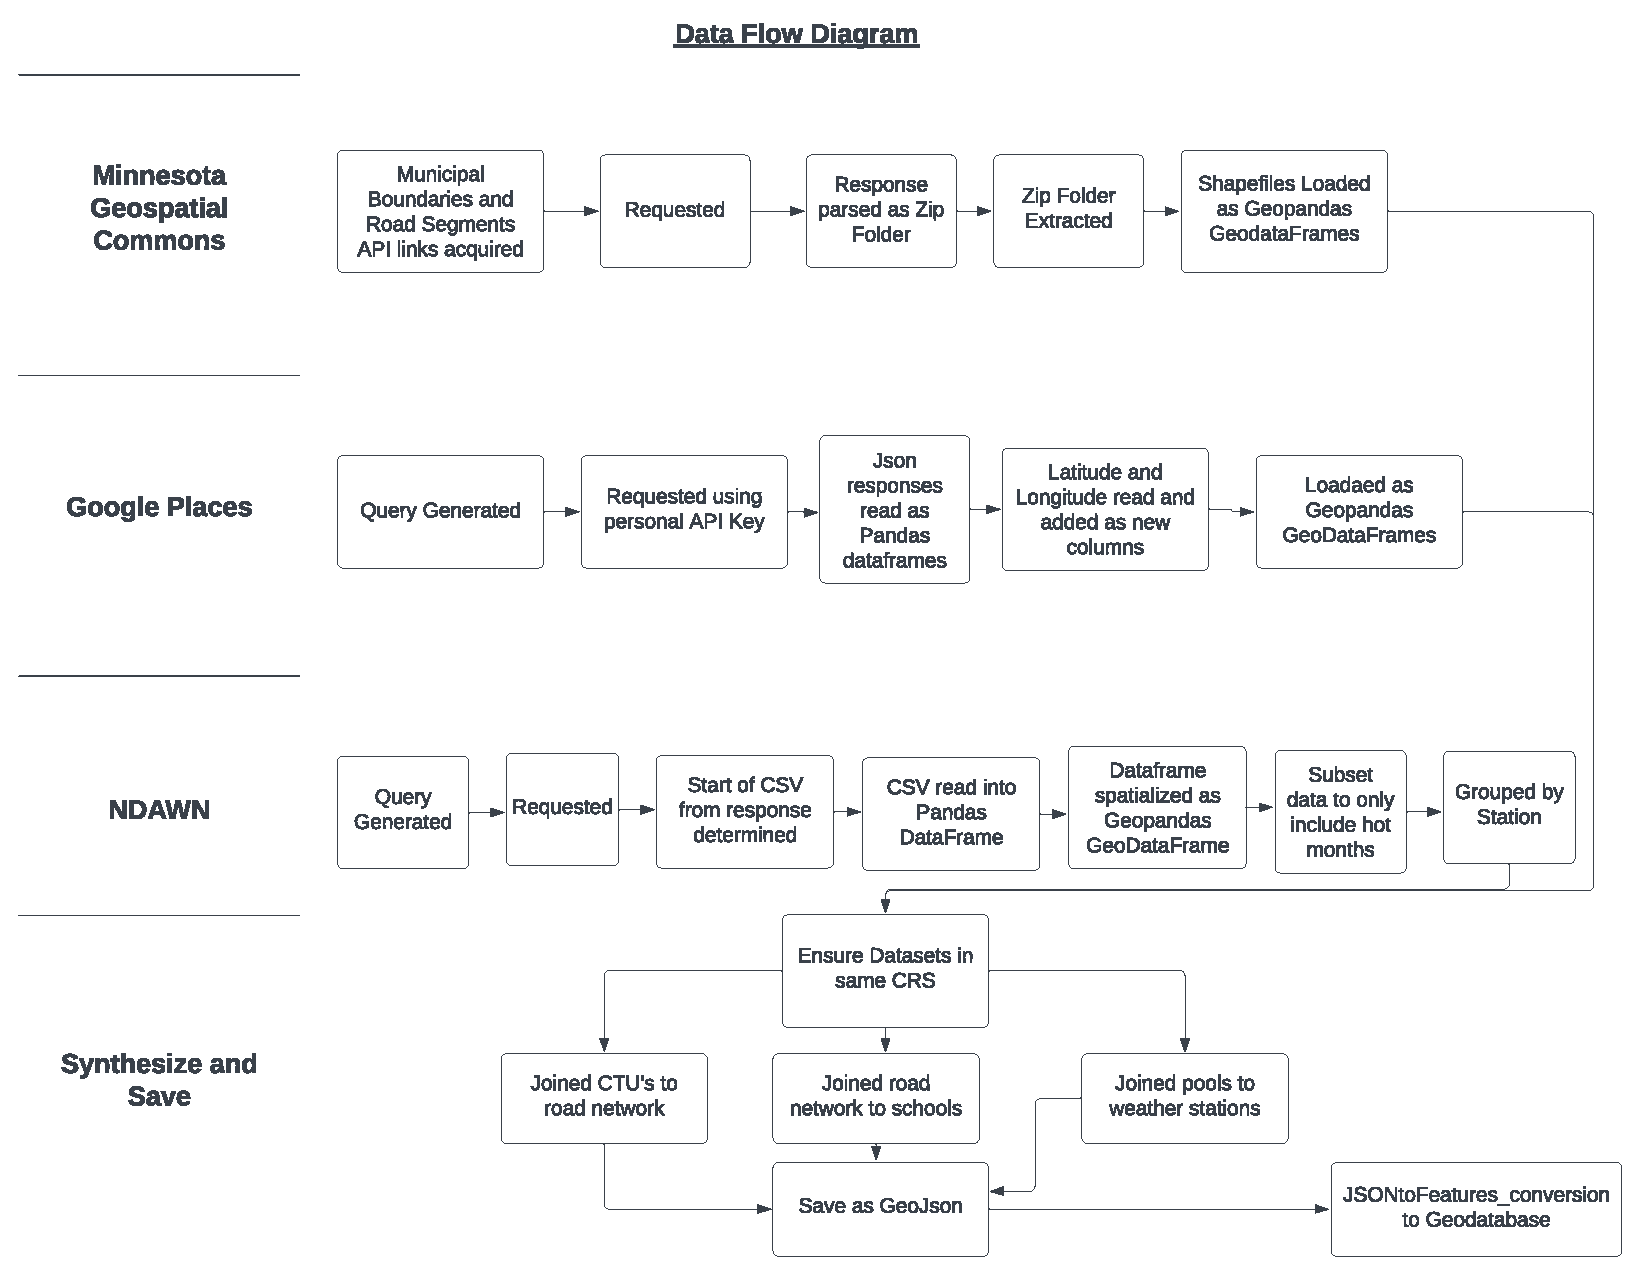
\includegraphics[width=\linewidth]{WorkFlow}
			\end{minipage}
			\captionof{figure}{Detailed Workflow}
		\end{center}
	\end{minipage}
}\\

\subsection*{Minnesota Geospatial Commons}

Geospatial Commons' API links can be found through their public facing website. Right clicking on the desired download link yields the desired url. This url can then be passed to a request library's "get" function where it can be parsed as a zip file. After extracting the contents of the zip file into the current working directory, the shapefiles within can be loaded into Geopandas as a GeoDataFrame. Code to perform these steps can be found in the following figure.
\\

\begin{adjustwidth}{-.7in}{-.7in}
	\fbox{ % Geospatial Commons Code
	\begin{minipage}{1\linewidth}
		\begin{center}
			\begin{minipage}{1\linewidth}
				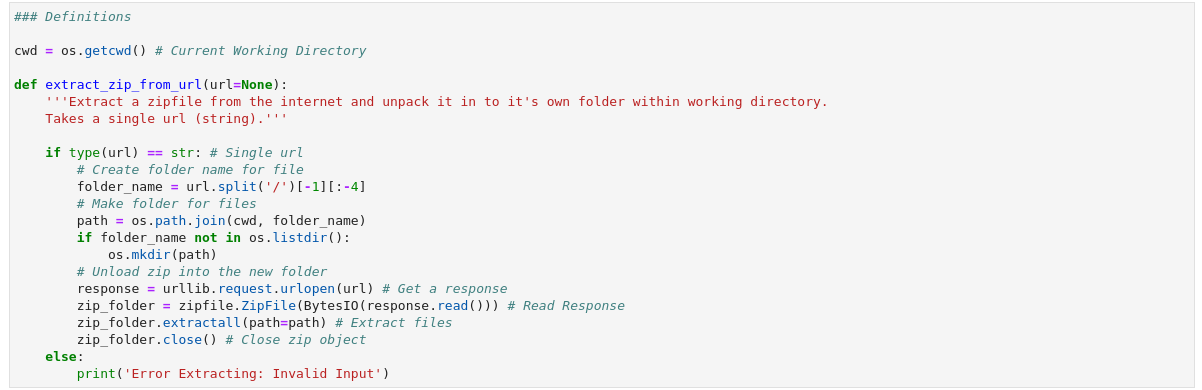
\includegraphics[width=\linewidth]{extractzip}
			\end{minipage}
			\\
			\begin{minipage}{1\linewidth}
				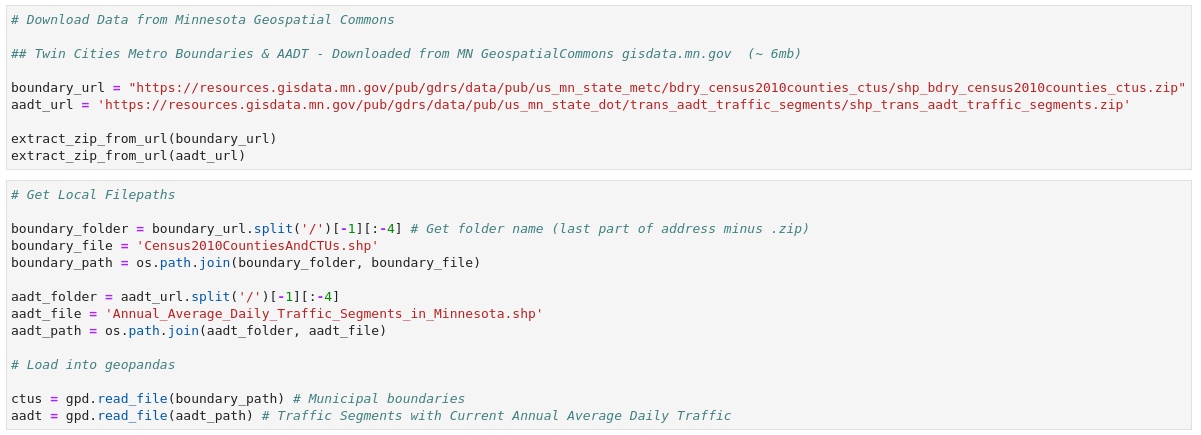
\includegraphics[width=\linewidth]{geocommonscode}
			\end{minipage}
			\captionof{figure}{Code to interface with Geocommons API}
		\end{center}
	\end{minipage}
}\\
\end{adjustwidth}

\subsection*{Google Places}

Google Places has extensive documentation on how to programatically query using their API. There are three options for Places querying: find place - for searching for a unique place, nearby search - for searching nearby a location, text search - for general queries based on a string. The format for their API url is: 

\begin{adjustwidth}{-.8in}{-.55in}
\small
\begin{verbatim}
https://maps.googleapis.com/maps/api/place/*search type*/json?inputs\&fields\&key=*API key*
\end{verbatim}
\end{adjustwidth}

After creating your own API key, you can develop your own queries. These queries can be requested and the responses can be read as dictionaries. Reading the dictionary as a Pandas DataFrame allows for easier manipulation. The latitude and longitude are within the dictionary in the geometry column under the location key. Once obtained, the DataFrame can be spatialized into a Geopandas GeoDataFrame using the points\_from\_xy function. Sample code is provided in the following figures. The first example is a nearby search of schools centered around the intersection of the 94 and 35W interstate highways. The second example searches for municipal pools in North Dakota with a location bias given as latitude, longitudes roughly correlating with the state of North Dakota.

\begin{adjustwidth}{-.7in}{-.7in}
	\fbox{ % Google API Code
		\begin{minipage}{1\linewidth}
			\begin{center}
				\begin{minipage}{1\linewidth}
					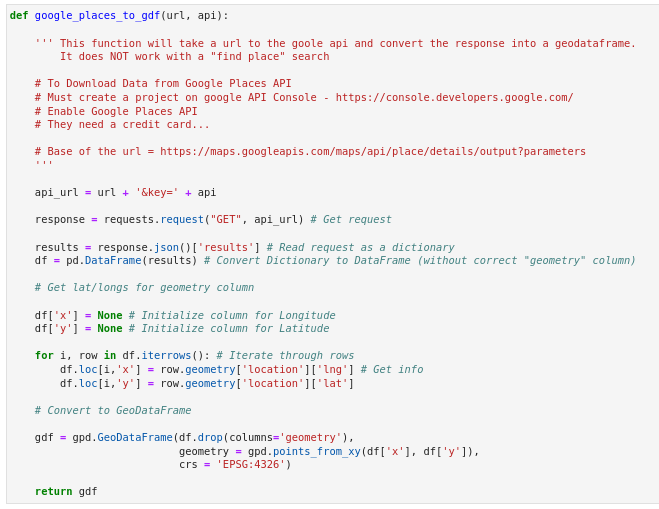
\includegraphics[width=\linewidth]{placestogdf}
				\end{minipage}
				\captionof{figure}{A function to interface with Google Places API}
			\end{center}
		\end{minipage}
	}\\
	\fbox{ % Google API Code
		\begin{minipage}{1\linewidth}
			\begin{center}
				\begin{minipage}{1\linewidth}
					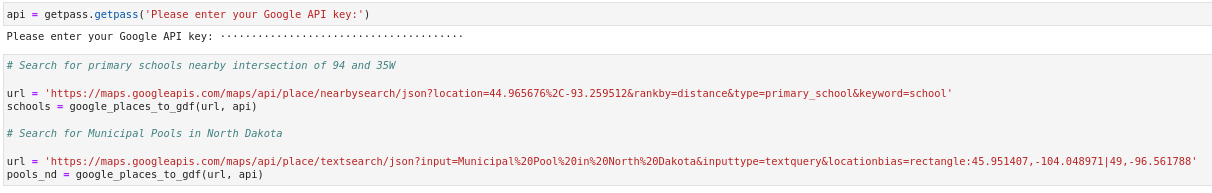
\includegraphics[width=\linewidth]{usingplacestogdf}
				\end{minipage}
				\captionof{figure}{Example queries with the Google Places API}
			\end{center}
		\end{minipage}
	}\\
\end{adjustwidth}


\subsection*{NDAWN}

The NDAWN API was easiest to interface with using their front facing website. After conducting the desired query, there is an 'Export CSV File' link at the top of the page that is the link to the API. An example of their API url is:


%\begin{adjustwidth}{-.8in}{-.55in}
	\small
	\begin{verbatim}
		https://ndawn.ndsu.nodak.edu/table.csv?station=40&variable=mdmxt
		&variable=mdmnt&variable=mdavt&year=2022&ttype=monthly&quick_pick=1_y
		&begin_date=2021-09&count=12
	\end{verbatim}
%\end{adjustwidth}

Which queries for the monthly maximum, minimum, and average temperatures of Minot, ND for the past year. The response from this is a CSV with a header describing the data and NDAWN. The first row of the CSV states the units of each column. This response can be decoded and read into a DataFrame. Latitude and longitude columns are provided so this DataFrame can be spatialized using the Geopandas points\_from\_xy function. 

Sample code that interfaces with this API is provided in the following figure. It gets the monthly minimum, maximum, and average temperatures across all stations in their system for the past year. Because each station must be explicitly stated, the url for this example is quite long, but it can be found in table 2. After getting the data into a GeoDataFrame, it was further subset for "pool-worthy months" defined as being above 80 degrees Fahrenheit, grouped by station, and pool-worthy months were saved as lists within a new GeoDataFrame.

\begin{adjustwidth}{-.7in}{-.7in}
	\fbox{ % ndawn API Code
		\begin{minipage}{1\linewidth}
			\begin{center}
				\begin{minipage}{1\linewidth}
					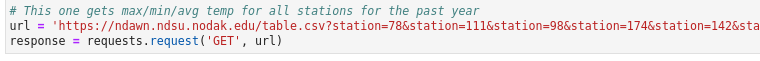
\includegraphics[width=\linewidth]{getndawn}
				\end{minipage}
				\captionof{figure}{Getting a response from the NDAWN API}
			\end{center}
		\end{minipage}
	}\\
	\fbox{ % ndawn API Code
		\begin{minipage}{1\linewidth}
			\begin{center}
				\begin{minipage}{1\linewidth}
					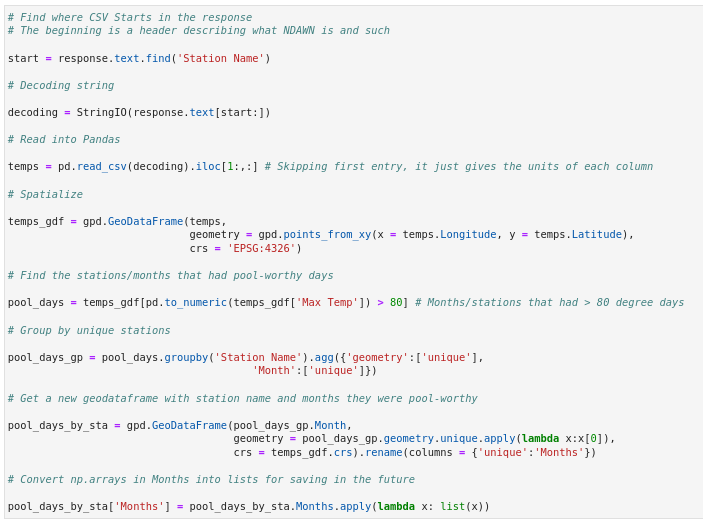
\includegraphics[width=\linewidth]{processndawn}
				\end{minipage}
				\captionof{figure}{Processing a response from the NDAWN API}
			\end{center}
		\end{minipage}
	}\\
\end{adjustwidth}

\subsection*{Synthesizing}

To synthesize the data each dataset was ensured to be in the same coordinate reference system (CRS). The roads and CTU's were in EPSG:26915 (UTM 15N) and the others were in EPSG:4326 (WGS84). The roads and CTU's were spatially joined so each road had information on the city or township it was in. The schools were joined to their nearest road segment so we could see the traffic volume nearby. The pool-worthy weather stations were joined to the nearest municipal pool to include in weather reports for hot days. Code that accomplishes this is provided in the following figures.

\begin{adjustwidth}{-.7in}{-.7in}
	\fbox{ % Google API Code
		\begin{minipage}{1\linewidth}
			\begin{center}
				\begin{minipage}{1\linewidth}
					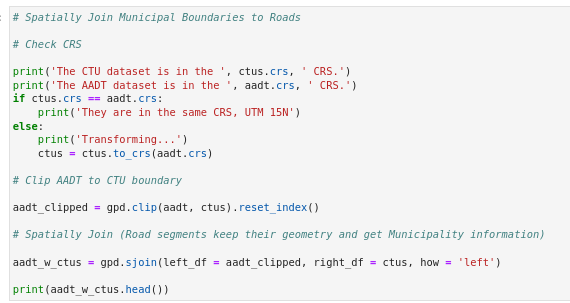
\includegraphics[width=\linewidth]{ctutoroad}
				\end{minipage}
				\captionof{figure}{Spatially joining CTU's to roads}
			\end{center}
		\end{minipage}
	}\\
	\fbox{ % Google API Code
		\begin{minipage}{1\linewidth}
			\begin{center}
				\begin{minipage}{.7\linewidth}
					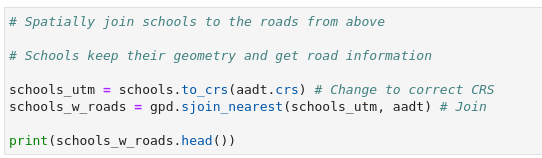
\includegraphics[width=\linewidth]{roadtoschool}
				\end{minipage}
				\captionof{figure}{Spatially joining roads to schools}
			\end{center}
		\end{minipage}
	}\\
	\fbox{ % Google API Code
		\begin{minipage}{1\linewidth}
			\begin{center}
				\begin{minipage}{\linewidth}
					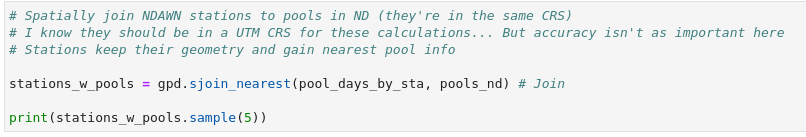
\includegraphics[width=\linewidth]{pooltostation}
				\end{minipage}
				\captionof{figure}{Spatially joining pools to weather stations}
			\end{center}
		\end{minipage}
	}\\
\end{adjustwidth}

\subsection*{Saving}

The results from the spatial joins were saved as GeoJson which were converted into the geodatabase of this project for visualization in ArcPro. These steps are given in the following figures.

\begin{adjustwidth}{-.7in}{-.7in}
	\fbox{
		\begin{minipage}{1\linewidth}
			\begin{center}
				\begin{minipage}{1\linewidth}
					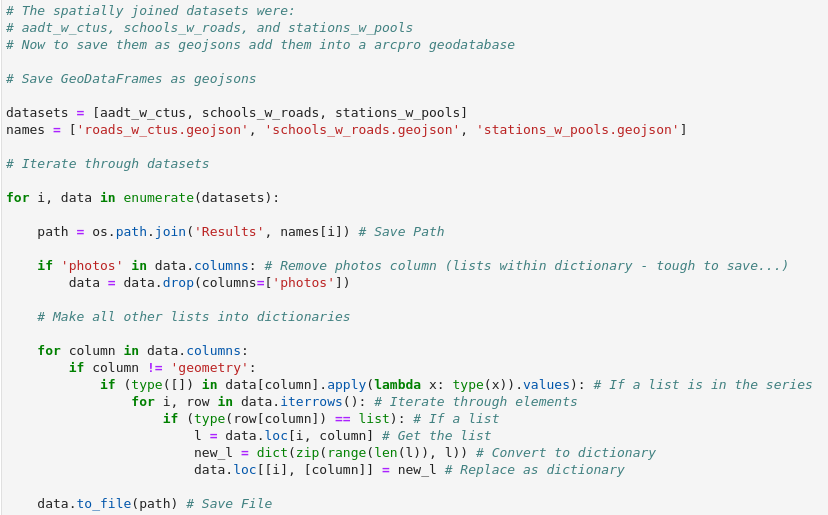
\includegraphics[width=\linewidth]{savetogeojson}
				\end{minipage}
				\captionof{figure}{Code to save the joined datasets to GeoJsons.}
			\end{center}
		\end{minipage}
	}\\
	\fbox{
		\begin{minipage}{1\linewidth}
			\begin{center}
				\begin{minipage}{\linewidth}
					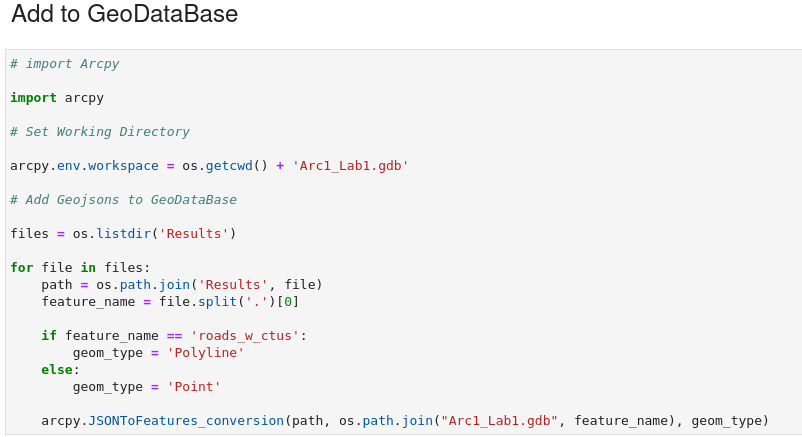
\includegraphics[width=\linewidth]{savetogdb}
				\end{minipage}
				\captionof{figure}{Code to save the GeoJsons to the project geodatabase}
			\end{center}
		\end{minipage}
	}\\
\end{adjustwidth}

\section*{Results}

\begin{adjustwidth}{-.7in}{-.7in}
	\fbox{ 
		\begin{minipage}{1\linewidth}
			\begin{center}
				\begin{minipage}{1\linewidth}
					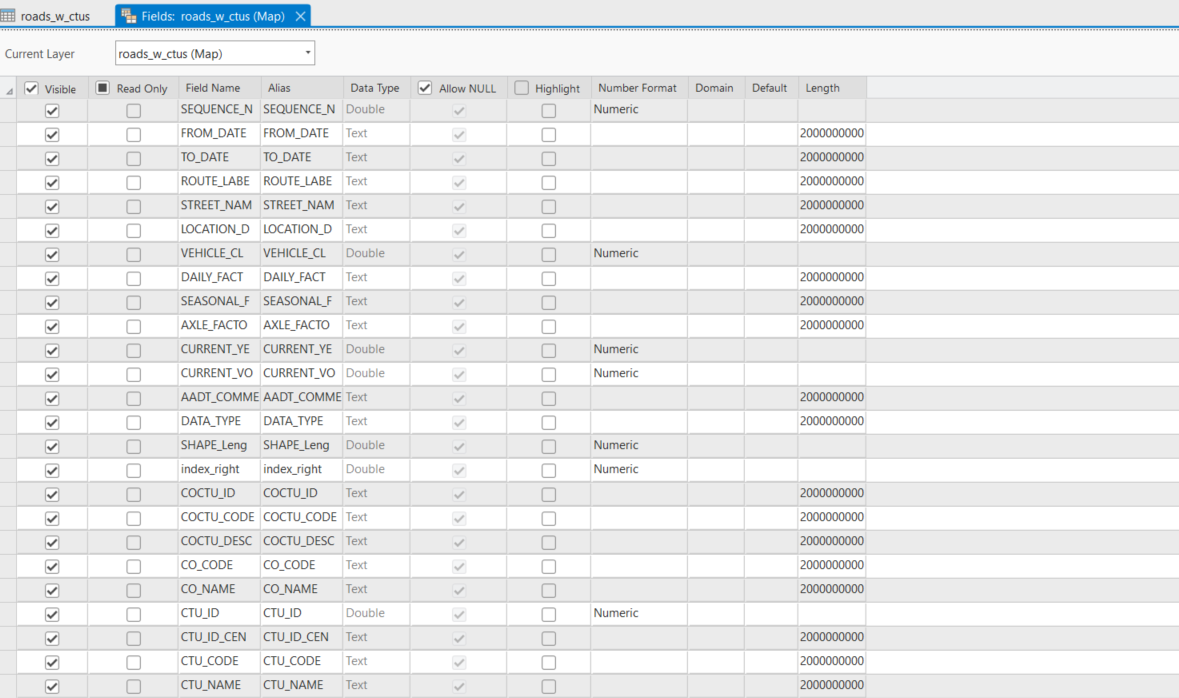
\includegraphics[width=\linewidth]{roadsandctu_fields}
				\end{minipage}
				\captionof{figure}{Fields view of CTU's joined to roads}
			\end{center}
		\end{minipage}
	}\newpage
	\fbox{ 
		\begin{minipage}{1\linewidth}
			\begin{center}
				\begin{minipage}{\linewidth}
					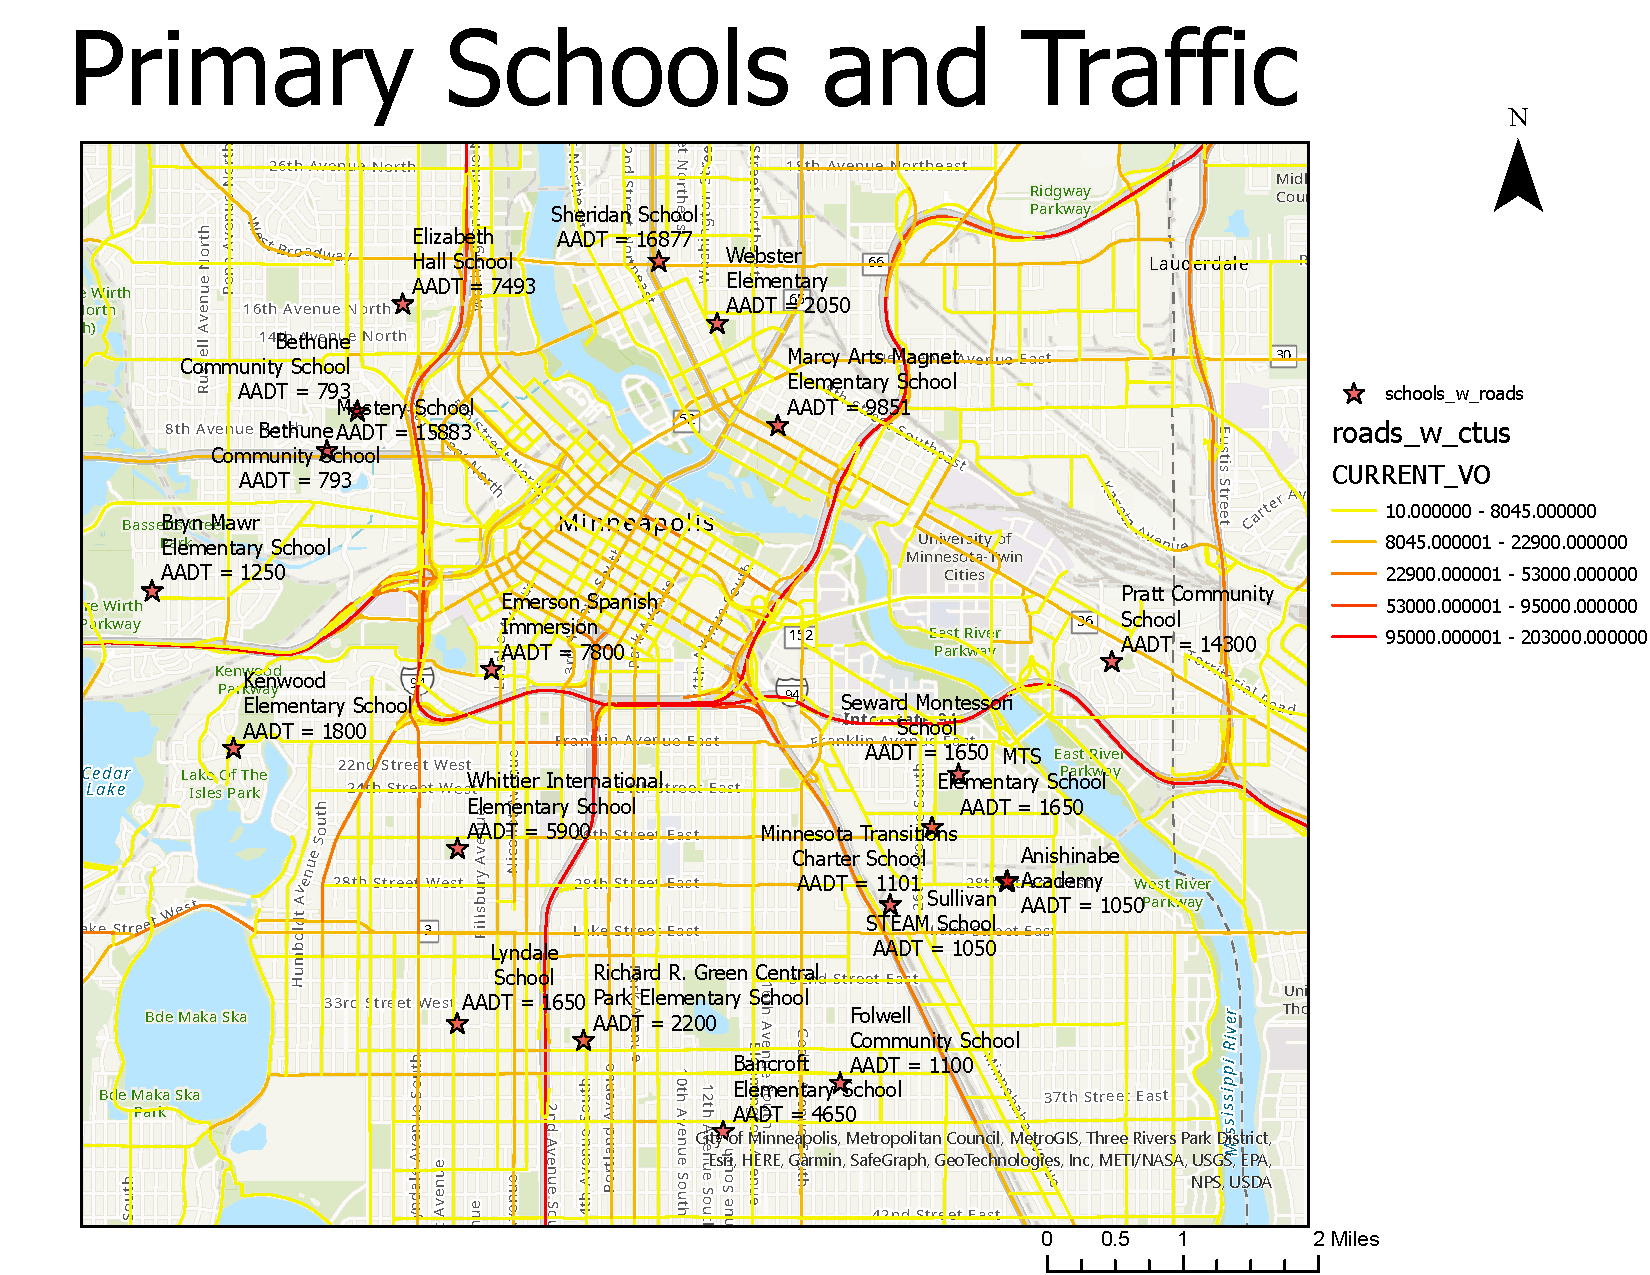
\includegraphics[width=.95\linewidth]{roads_w_schools}
				\end{minipage}
				\captionof{figure}{Visualization of roads and schools. School labels include AADT of their nearest road.}
			\end{center}
		\end{minipage}
	}\\
	\fbox{ 
		\begin{minipage}{1\linewidth}
			\begin{center}
				\begin{minipage}{\linewidth}
					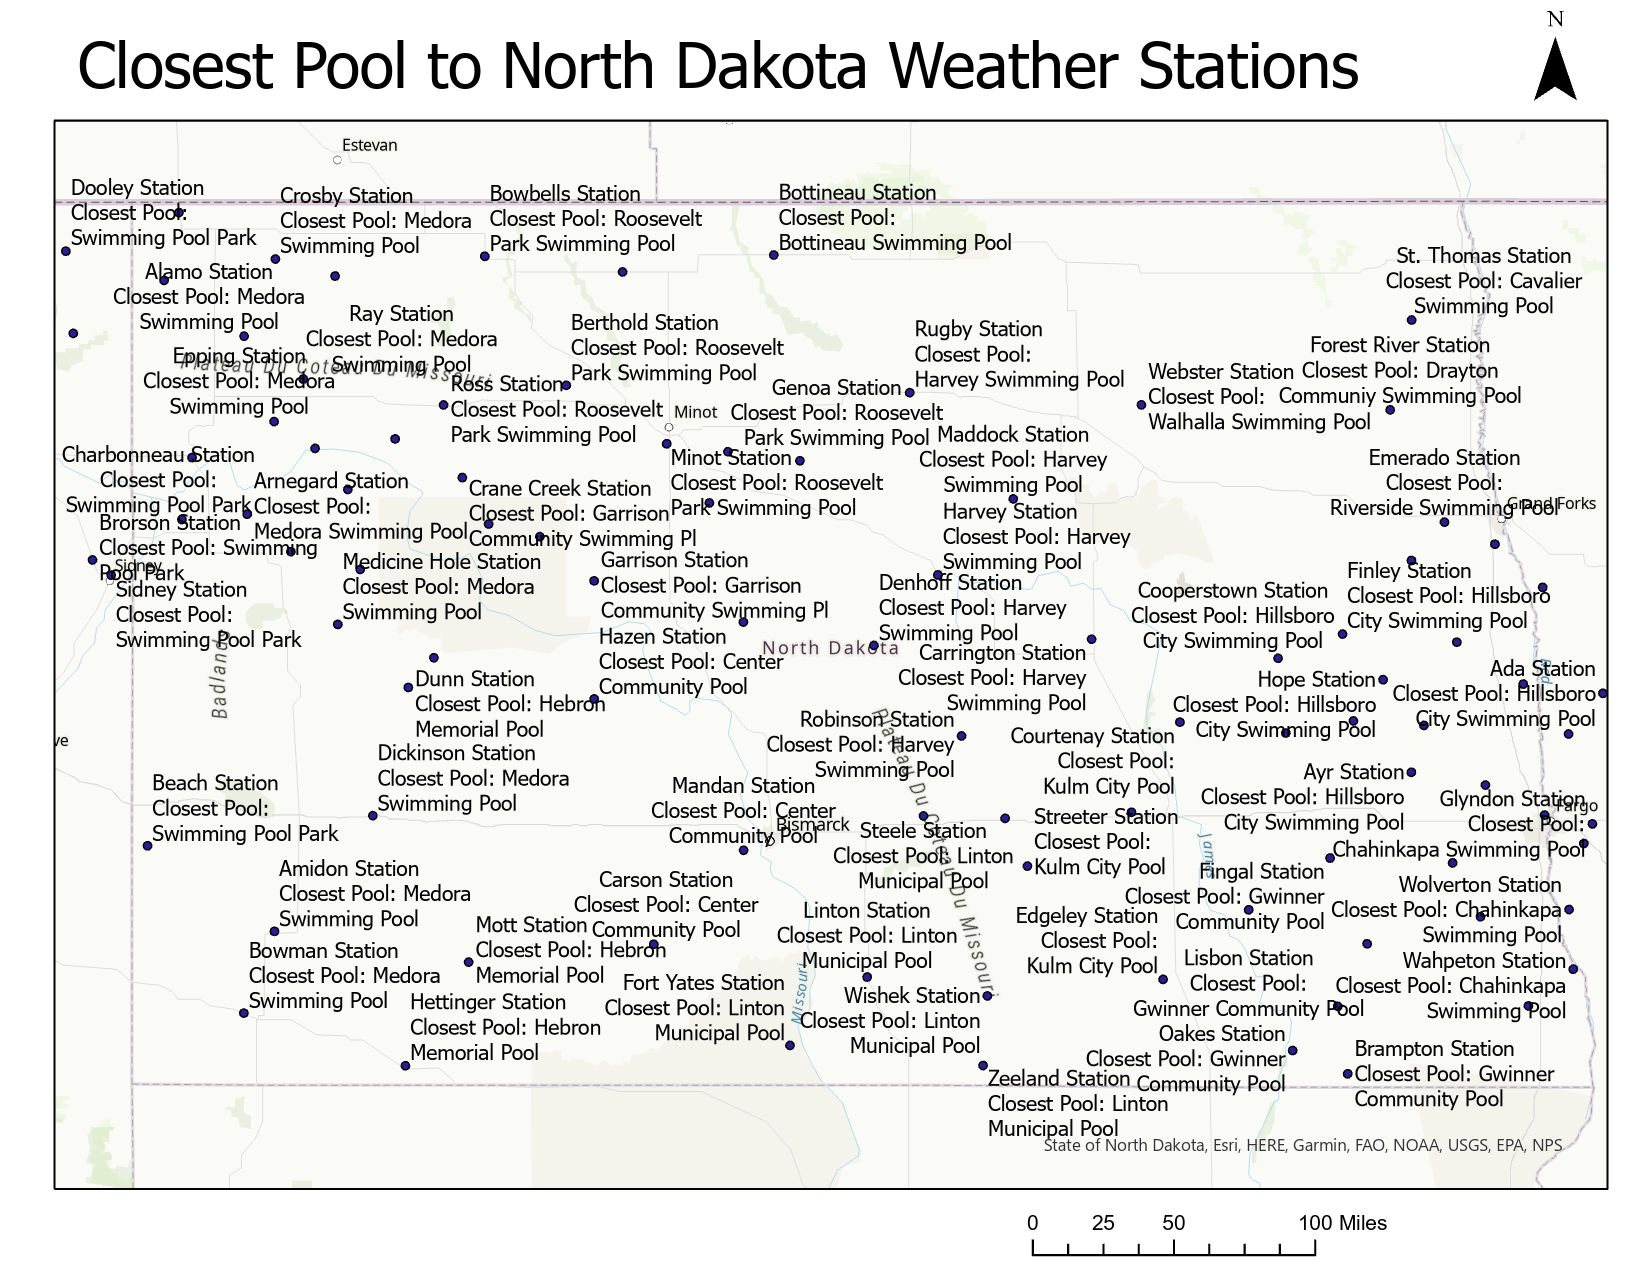
\includegraphics[width=\linewidth]{nd_pools}
				\end{minipage}
				\captionof{figure}{Visualization of North Dakota weather stations. Labels include nearest pool to each station.}
			\end{center}
		\end{minipage}
	}\\
\end{adjustwidth}

Visually, we can see that the results across all datasets are in the correct locations and have the appropriate fields.

\section*{Discussion and Conclusion}

Through this lab I was able to explore how to programatically interact with three very different API's. 

The Minnesota Geospatial Commons API provides data in a familiar spatial format (shapefiles). The naming conventions across the API, however, do not appear very standardized. This would make each request rather unique and someone needing to access multiple datasets would likely need to navigate their website first to develop a list of their API urls.

Google Places has pretty good documentation and standardized querying conventions. It would be quite easy to develop a flexible ETL workflow that can handle a wide variety of requests. The trouble is that you need to have an API key to perform queries which involves supplying a credit card and, potentially, a bill!

NDAWN's API was similar to Google Places in how it was structured and an ETL workflow  handling a variety of requests could be developed. There was no real documentation that I could find, however, and they used a few abbreviations that were incomprehensible without performing a few requests manually.

Upon completing this lab, I am much more confident interfacing with API's and feel ready to begin to develop some ETL's for my project!  

%\begingroup           % Ctrl T to uncomment
%\setstretch{1}
%\setlength\bibitemsep{12pt}  % length between two different entries
%\printbibliography
%\endgroup

\section*{Self Score}
\setstretch{.2}
\begin{tabular}{|p{.2\linewidth}|p{.2\linewidth}|p{.2\linewidth}|p{.1\linewidth}|}
	\hline
	\textbf{Category}            & \textbf{Description}                                                                                                                                                                                                                                                                                                                                              & \textbf{Points Possible} & \textbf{Score} \\ \hline
\vspace{.2in}\textbf{Structural Elements} & {\tiny All elements of a lab report are included (2 points each): Title, Notice: Dr. Bryan Runck, Author, Project Repository, Date, Abstract, Problem Statement, Input Data w/ tables, Methods w/ Data, Flow Diagrams, Results, Results Verification, Discussion and Conclusion, References in common format, Self-score}                                        & \vspace{.2in}28              &   \vspace{.2in}22    \\ \hline
	\vspace{.2in}\textbf{Clarity of Content}  & {\tiny Each element above is executed at a professional level so that someone can understand the goal, data, methods, results, and their validity and implications in a 5 minute reading at a cursory-level, and in a 30 minute meeting at a deep level (12 points). There is a clear connection from data to results to discussion and conclusion (12 points).} & \vspace{.2in}24              &  \vspace{.2in}20     \\ \hline
	\vspace{.2in}\textbf{Reproducibility}     & {\tiny Results are completely reproducible by someone with basic GIS training. There is no ambiguity in data flow or rationale for data operations. Every step is documented and justified.}                                                                                                                                                                     & \vspace{.2in}28              &     \vspace{.2in}28  \\ \hline
	\vspace{.2in}\textbf{Verification}        & {\tiny Results are correct in that they have been verified in comparison to some standard. The standard is clearly stated (10 points), the method of comparison is clearly stated (5 points), and the result of verification is clearly stated (5 points).}                                                                                                      & \vspace{.2in}20              &   \vspace{.2in}10   \\ \hline
	&                                                                                                                                                                                                                                                                                                                                                          & \vspace{.02in}100             &   \vspace{.02in}80     \\ \hline
\end{tabular}
\end{document}